\section{Optics}\label{ssec:optics}
The receiver optics are a good place to start of with, because the optics are not very dependent on results achieved in other areas. The optics have to transport as many desired photons, and as little unwanted photons to the active area on the SPADs as possible. All while having an acceptable depth of field. 

The most basic solution is a single lens with an aperture. The opacity of the lens can be calculated with the absorption of the lens material and f-number of the lens using \cref{eq:basic_opacity}.

\begin{align}\label{eq:basic_opacity}
\text{opacity} = \frac{1-\text{absorption}}{\text{f-number}^2}
\end{align}

 The performance of a possible configuration is shown in \cref{tab:basic_optics}

\begin{table}[H]
\centering
\caption{Performance of basic optics solution}
\label{tab:basic_optics}
\begin{tabular}{|l|r|}\hline
    \textbf{Basic Optics} & \\
    \hline 
    f-number & $2.00\, $ \\
    absorption & $5.00\,\%$ \\
    opacity & $23.75\, \%$ \\
    \hline 
\end{tabular}
\end{table}


\subsection{Improvements}
There are a couple of additions that can improve the performance of the optics. The first and essential one, is the use of a bandpass filter. The transmitted signal will have a very specific bandwidth of $850\,nm$. Using a narrow bandpass filter one can filter out an enormous part of the background noise. The filter will have an opacity of $50\,\%$ for the target wavelength.

The captured photons that hit the lens need to be guided to the active area of the SPADs. If the active area on the chip is very small, one can use microlenses to improve the effectiveness of the optics. A Microlens focuses light on a single SPAD on the chip. Two types of microlenses will be considered: a spherical lens, and a square shaped lens. The presence of microlenses poses a limitation of the main lens. The f-number must be relatively large. A higher f-number means a smaller aperture and therefore more loss of photons. A way of dealing with this problem is to use a second lens instead. An overview of the available options is shown in \cref{tkz:receiver_optics}

\begin{figure}[H]
    \centering


\resizebox{\linewidth*3/4}{!}{
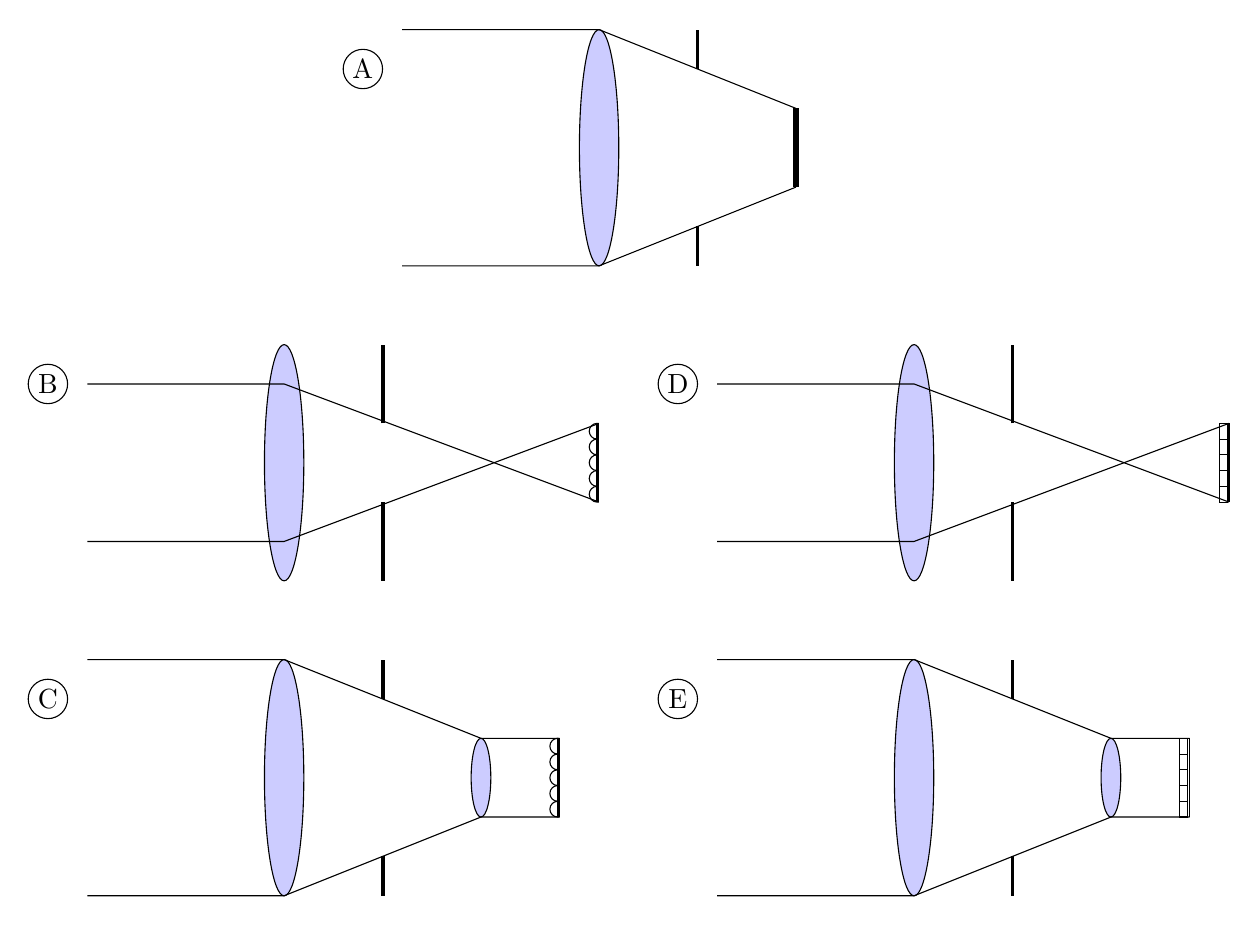
\begin{tikzpicture}[scale=.5]

%%%%%% low F-number, no microlens

%lens
\draw [fill=blue!20] (7,4) ellipse (0.5 and 3);

%diafragma
\draw [line width=.5mm] (9.5,6) -- (9.5,7);
\draw [line width=.5mm] (9.5,1) -- (9.5,2);

%sensitive area
\draw [line width=.7mm] (12,3) -- (12,5);

%light beams
\draw (2,7) to (7,7) to (12,5);
\draw (2,1) to (7,1) to (12,3);

%%%%%%Microlens + high F-number

%lens
\draw [fill=blue!20] (-1,-4) ellipse (0.5 and 3);

%diafragma
\draw [line width=.5mm] (1.5,-3) -- (1.5,-1);
\draw [line width=.5mm] (1.5,-7) -- (1.5,-5);

%sensitive area
\draw [line width=.7mm] (7,-5) -- (7,-3);

%light beams
\draw (-6,-2) to (-1,-2) to (7,-5);
\draw (-6,-6) to (-1,-6) to (7,-3) node (v1) {};


%Microlenses
\draw  (6.95,-3.2) ellipse (.2 and .2);
\draw  (6.95,-3.6) ellipse (.2 and .2);
\draw  (6.95,-4.0) ellipse (.2 and .2);
\draw  (6.95,-4.4) ellipse (.2 and .2);
\draw  (6.95,-4.8) ellipse (.2 and .2);
\fill  (7,-2.8) rectangle (7.4,-5.2) [fill=white];

%%%%%%Microlens + extra lens

%lens
\draw [fill=blue!20] (-1,-12) ellipse (0.5 and 3);

%second lens
\draw [fill=blue!20] (4,-12) ellipse (0.25 and 1);

%diafragma
\draw [line width=.5mm] (1.5,-10) -- (1.5,-9);
\draw [line width=.5mm] (1.5,-15) -- (1.5,-14);

%sensitive area
\draw [line width=.75mm] (6,-13) -- (6,-11);

%light beams
\draw (-6,-9) to (-1,-9) to (4,-11) to (6,-11);
\draw (-6,-15) to (-1,-15) to (4,-13) to (6,-13);


%Microlenses
\draw  (5.95,-11.2) ellipse (.2 and .2);
\draw  (5.95,-11.6) ellipse (.2 and .2);
\draw  (5.95,-12) ellipse (.2 and .2);
\draw  (5.95,-12.4) ellipse (.2 and .2);
\draw  (5.95,-12.8) ellipse (.2 and .2);
\fill  (6,-10.8) rectangle (6.4,-13.2) [fill=white];

%%%%%% Square Microlens + high F-number

%lens
\draw [fill=blue!20] (15,-4) ellipse (0.5 and 3);

%diafragma
\draw [line width=.5mm] (17.5,-3) -- (17.5,-1);
\draw [line width=.5mm] (17.5,-7) -- (17.5,-5);

%sensitive area
\draw  (23,-5) -- (23,-3);

%light beams
\draw (10,-2) to (15,-2) to (23,-5);
\draw (10,-6) to (15,-6) to (23,-3);


%Microlenses
\draw  (22.75,-3) rectangle (22.95,-3.4);
\draw  (22.75,-3.4) rectangle (22.95,-3.8);
\draw  (22.75,-3.8) rectangle (22.95,-4.2);
\draw  (22.75,-4.2) rectangle (22.95,-4.6);
\draw  (22.75,-4.6) rectangle (22.95,-5);


%%%%%% Square Microlens + extra lens

%lens
\draw [fill=blue!20] (15,-12) ellipse (0.5 and 3);

%second lens
\draw [fill=blue!20] (20,-12) ellipse (0.25 and 1);

%diafragma
\draw [line width=.5mm] (17.5,-10) -- (17.5,-9);
\draw [line width=.5mm] (17.5,-15) -- (17.5,-14);

%sensitive area
\draw  (22,-13) -- (22,-11);

%light beams
\draw (10,-9) to (15,-9) to (20,-11) to (22,-11);
\draw (10,-15) to (15,-15) to (20,-13) to (22,-13);


%Microlenses
\draw  (21.75,-11) rectangle (21.95,-11.4);
\draw  (21.75,-11.4) rectangle (21.95,-11.8);
\draw  (21.75,-11.8) rectangle (21.95,-12.2);
\draw  (21.75,-12.2) rectangle (21.95,-12.6);
\draw  (21.75,-12.6) rectangle (21.95,-13);



\draw  (1,6) ellipse (.5 and .5) node[]{A};
\draw  (-7,-2) ellipse (.5 and .5) node[]{B};
\draw  (-7,-10) ellipse (.5 and .5) node[]{C};
\draw  (9,-2) ellipse (.5 and .5) node[]{D};
\draw  (9,-10) ellipse (.5 and .5) node[]{E};


\end{tikzpicture}
}

    \caption{Overview of possible receiver optics implementations}
    \label{tkz:receiver_optics}
\end{figure}

\begin{align}
\text{opacity} = (1-\text{absorption}_1)(1-\text{absorption}_2)\cdot\text{opacity filter}\cdot \frac{X}{\text{f-number}^2}
\end{align}
Where $X$ is the active area on the chip. A comparison between the different options is shown in \cref{tab:receiver_optics}

\begin{table}[H]
\centering
\caption{comparison of different optics solutions}
\label{tab:receiver_optics}
\begin{tabular}{|l|lllll|}\hline
\textbf{Type}                & \textbf{A}        & \textbf{B}        & \textbf{C}        & \textbf{D}        & \textbf{E}        \\ \hline
absorption $1^{st}$ lens & 0.05     & 0.05     & 0.05     & 0.05     & 0.05     \\
f-number                 & 2        & 8        & 2        & 8        & 2        \\
absorption $2^{nd}$ lens & 0        & 0        & 0.05     & 0        & 0.05     \\
active area on chip      & 0.05     & 0.55     & 0.55     & 0.65     & 0.65     \\ \hline
effective opacity            & 0.011875 & 0.008164 & 0.124094 & 0.009648 & 0.146656 \\ \hline
\end{tabular}
\end{table}

The comparison in \cref{tab:receiver_optics} shows some good alternatives to the basic lens, if there is a need for it due to a small active area on the chip. However, most of the future calculations will focus on the basic model A.

